\documentclass[a4paper,oneside]{memoir}
\usepackage[english]{babel}
\usepackage[T1]{fontenc}
\usepackage[utf8]{inputenc}
\usepackage{wallpaper}
\usepackage{palatino}
\usepackage{listings}
\usepackage{hyperref}
\usepackage{float}
\usepackage{subcaption}
\hypersetup{
    colorlinks=true,
    linkcolor=blue,
    filecolor=magenta,      
    urlcolor=cyan,
}
\counterwithout{section}{chapter}
% Setup captions
%\captionstyle[\centering]{\centering}
%\changecaptionwidth
%\captionwidth{0.8\linewidth}

% Protect against widows and orphans
%\clubpenalty=10000
%\widowpenalty=10000

%\linespread{1.2}

%\raggedbottom

%\chapterstyle{ger}

%\maxsecnumdepth{subsection}

\lstset{language=C,
                basicstyle=\ttfamily,
                keywordstyle=\color{blue}\ttfamily,
                stringstyle=\color{red}\ttfamily,
                commentstyle=\color{green}\ttfamily,
                morecomment=[l][\color{magenta}]{\#}
}

%%  Setup fancy style quotation
%%  ==================================================================
%\usepackage{tikz}
%\usepackage{framed}

%\newcommand*\quotefont{\fontfamily{fxl}} % selects Libertine for quote font

% Make commands for the quotes
%\newcommand*{\openquote}{\tikz[remember picture,overlay,xshift=-15pt,yshift=-10pt]
%     \node (OQ) {\quotefont\fontsize{60}{60}\selectfont``};\kern0pt}
%\newcommand*{\closequote}{\tikz[remember picture,overlay,xshift=15pt,yshift=5pt]
%     \node (CQ) {\quotefont\fontsize{60}{60}\selectfont''};}

% select a colour for the shading
%\definecolor{shadecolor}{rgb}{1,1,1}

% wrap everything in its own environment
%\newenvironment{shadequote}% 
%{\begin{snugshade}\begin{quote}\openquote}
%{\hfill\closequote\end{quote}\end{snugshade}}

%%  Begin document
%%  ==================================================================
\begin{document}

%%  Begin title page
%%  ==================================================================
    \thispagestyle{empty}
    \ULCornerWallPaper{1}{ku-coverpage/diku-en.pdf}
    \ULCornerWallPaper{1}{ku-coverpage/diku-en.pdf}
    \begin{adjustwidth}{-3cm}{-1.5cm}
    \vspace*{-1cm}
    \textbf{\Huge Project outside course scope} \\
    \vspace*{2.5cm} \\
    \textbf{\Huge Accelerating Ocean Modelling} \\
    \vspace*{.1cm} \\
    {\huge Adressing performance bottlenecks of the ocean modelling framework Veros} \\
    \begin{tabbing}
    % adjust the hspace below for the longest author name
    Till Grenzdörffer \hspace{1cm} \= \texttt{vmt184@alumni.ku.dk} \\
    \\[12cm]
    \textbf{\Large Supervisor} \\
    Cosmin Eugen Oancea \> \texttt{cosmin.oancea@di.ku.dk} \\
    \end{tabbing}
    \end{adjustwidth}
    \newpage
    \ClearWallPaper



%%  ==================================================================
%%  End title page
\section{Introduction}
Currently many scientists are using purely sequential software for ocean modelling, leading to long simulation times and inefficient use of modern hardware. 
The aim of this project is to tackle this problem by introducing and optimizing highly parallel code that uses the potential of modern GPUs to accelerate the modelling process.

The ocean modelling framework this project is based on is Veros \cite{veros}. It is written in python and uses Jax \cite{jax2018github} to parallelize large parts of the computations.
However, there is reason to believe that the parallel code generated by Jax (specifically on GPUs) is not optimal and warrants the implementation of specific bottlenecks in a language like CUDA, possibly generated by Futhark.

Another part of this project is the integration of CUDA code into Jax through XLA calls.
This allows an easy use of the parallel code through a python interface.


\section{Tridiagonal Solver}
In this project I first investigated the implementation of a tridiagonal solver that is used throughout Veros. 
The requirement for this solver is that it solves many (ca. 50000) tridiagonal systems with comparably small diagnonals (ca. 100) as fast as possible.

I considered two algorithms for solving tridiagonal systems for this task and experimented with different performance optimizations for both.

\subsection{Thomas Algorithm}
One simple algorithm for solving a tridiagonal system is the Thomas Algorithm.
Pythonlike pseudocode for it is shown in fig.~\ref{fig:thomas}.
We can see that in the both for-loops there are true RAW-dependencies across iterations, which means that the algorithm itself is not trivially parallelizable.
However, in our case we want to solve many small tridiagonal systems, so we can parallelize over the different systems and leave the Thomas Algorithm in its sequential form.
As long as we have enough systems to fully utilize the GPU it is running on, this implementation seems like a good approach.

\begin{figure}[hbtp]
    \caption{Thomas algorithm in pythonlike pseudocode}
    \label{fig:thomas}
    \begin{lstlisting}[language=python,frame=single]
for i in range(1, n):
    w = a[i] / b[i - 1]
    b[i] += -w * c[i - 1]
    d[i] += -w * d[i - 1]

out[-1] = d[-1] / b[-1]

for i in range(n - 2, -1, -1):
    out[i] = (d[i] - c[i] * out[i + 1]) / b[i]
    \end{lstlisting}
\end{figure}


\subsection{Thomas Algorithm - Coalesced}
In the trivial algorithm, successive iterations of the recurrent loop access neighboring data in memory.
Since we assign one tridiagonal system to each thread, neighboring threads access data with the stride of the size of the tridiagonal system. This means that the accesses are uncoalesced and we can improve the performance significantly by changing the underlying data layout. 
In this case the change is trivial - we just need to transpose the input matrix, which can be done efficiently using shared-memory tiling and tranpose the result back afterwards. 

The benchmarks show clearly that the benefit of the transposition on the main kernel outweighs the cost of the transposition and thus increases the performance by a factor of XXXX.

\subsection{Thomas Algorithm - Loop unrolling}
Since in our use case the size of the tridiagonal systems is relatively small, it might make sense to unroll the recurrent loops. However, this is only possible if we know the size of the systems at compile time, or compile the CUDA kernel at runtime (for example using CuPy \cite{cupylearningsys2017}). 
However, I expect the benefit of this to be too small to warrant the significant overhead of JIT compilation.

\subsection{Flat version}
The flat version of the tridiagonal solver is based on the observation, 
that all recurrences in the Thomas algorithm can be replaced with a scan with an appropriate operator. 
For example, after inlining the computation of w and replacing the +=, we get the following line: 
\begin{verbatim}
    b[i] = b[i] - a[i] * c[i - 1] / b[i - 1] 
\end{verbatim}
As explained in \cite{andreetta2016finpar} in more detail, this statement matches the pattern $b_i = a_i + c_i / b_{i-1}$, which can be replaced with a scan that uses 2x2 matrix multiplication as its operator.
Similarly, the other recurrences can be replaced by a scan with linear function composition.

I implemented this flat algorithm in CUDA using the thrust library, which provides a scan implementation with custom operators on the GPU.
For comparison, I also included the Futhark implementation of the authors of \cite{andreetta2016finpar} from the 
\href{https://github.com/diku-dk/futhark-benchmarks/blob/bf5112d0841866dc7370586f2e2a7b48467d2d97/finpar/LocVolCalib.fut}{futhark benchmarks}
repository.

Compared to the Thomas algorithm, this algorithm is more computationally expensive, however if the size of the tridiagonal systems is large enough or we have sufficiently parallel hardware, the benefits of parallelization should outweigh the additional computational load. 

\subsection{Flat version - shared memory}
Since my initial implementation of the flat algorithm used thrust scans, the computation involved the launch of 6 kernels in total. This means that there are a lot of redundant accesses to global memory. 

In order to evaluate the effect of this, I also implemented a version of the flat algorithm that is computed completely within shared memory.

Here a block is assigned to each tridiagonal system (given that the system is not too large to fit shared memory), and the flat algorithm is computed using intra block scans. For this I used parts of the code handouts from the PMPH course.


\subsection{Precision}
In order to be useful, all of the implementations of course need to produce results that match a reference implementation. However, due to the nature of floating point computation, this will almost never be exact.

Interestingly, the error margin varied a lot between the algorithms. The flat implementations suffered far greater imprecision, probably at least partly due to the increased parallelism and thereby more indeterminstic order of execution, but also just due to the higher number of floating point calculations.

However, in Veros the tridiagonal systems this solver is supposed to work on are guaranteed to be diagonally dominant. Testing the algorithms on systems with this property showed that all algorithms produce meaningful results.
\subsection{Futhark}
In addition to the CUDA implementations, I also included a sequential and a flat implementation (from \href{https://github.com/diku-dk/futhark-benchmarks/blob/bf5112d0841866dc7370586f2e2a7b48467d2d97/finpar/LocVolCalib.fut}{futhark benchmarks}) in the benchmarks in order to see how close the high level description of the algorithms compiled by the futhark compiler will come to CUDA implementations that were optimized by hand.

\subsection{Benchmarks}

\vspace*{\fill}

\begin{figure}[H]
    \begin{subfigure}[b]{0.6\textwidth}
        \centering
        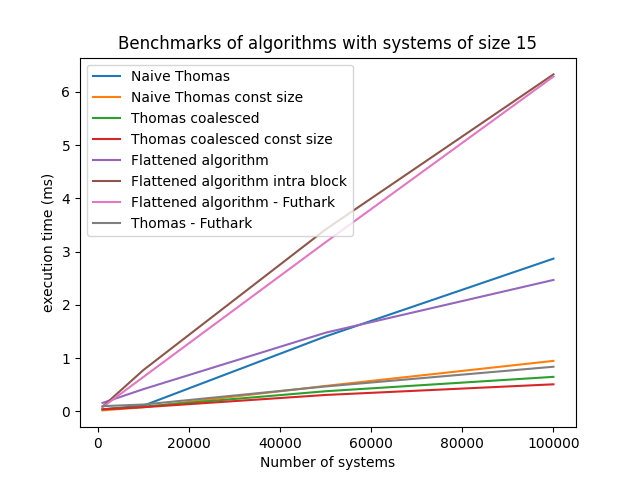
\includegraphics[width=\textwidth]{timings_15.png}
        \caption{Tridiagonal systems of size 15}
        \label{fig:bench15}
    \end{subfigure}
    % \hfill
    \begin{subfigure}[b]{0.6\textwidth}
        \centering
    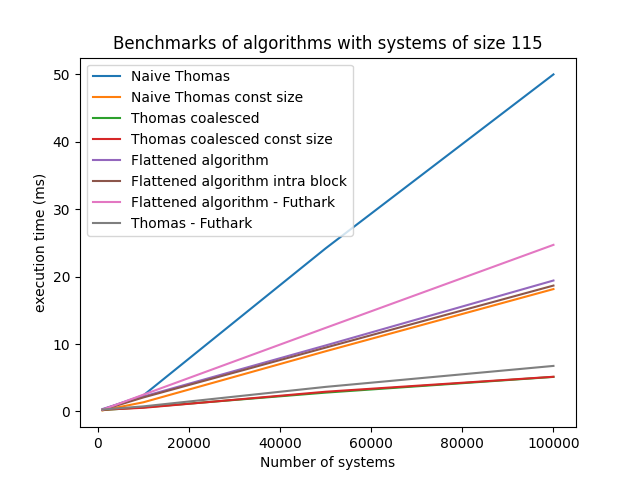
\includegraphics[width=\textwidth]{timings_115.png}
    \caption{Tridiagonal systems of size 115}
    \label{fig:bench115}
        \end{subfigure}
    % \vskip\baselineskip
    \begin{subfigure}[b]{0.6\textwidth}
        \centering
    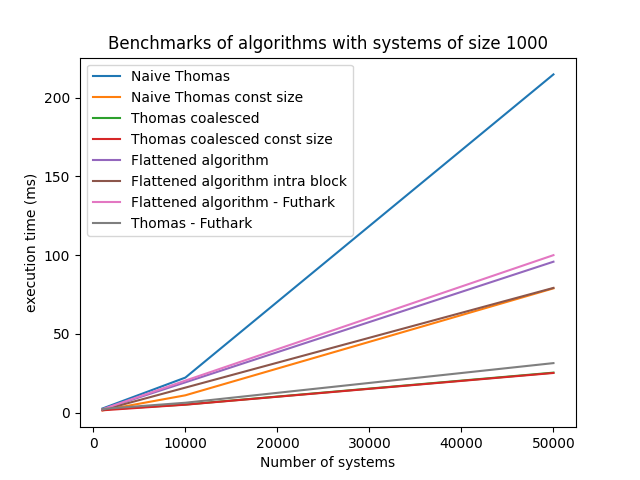
\includegraphics[width=\textwidth]{timings_1000.png}
    \caption{Tridiagonal systems of size 1000}
    \label{fig:bench1000}
    \end{subfigure}
    % \hfill
    \begin{subfigure}[b]{0.6\textwidth}
        \centering
    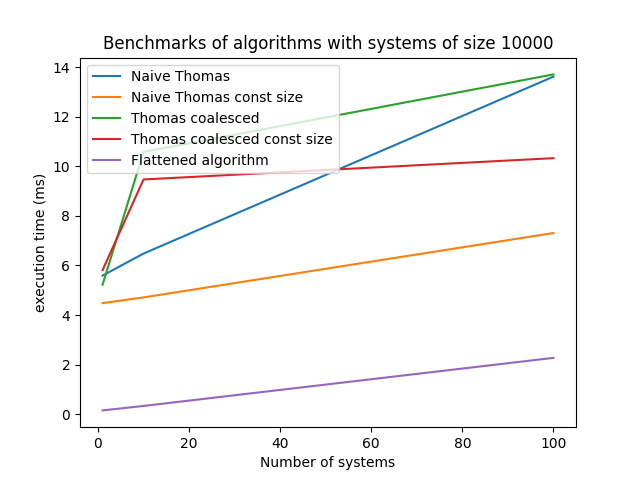
\includegraphics[width=\textwidth]{timings_10000.png}
    \caption{Tridiagonal systems of size 10000}
    \label{fig:bench10000}
    \end{subfigure}
    
 \end{figure}

The performance of the different algorithms are shown in figs.~\ref{fig:bench15}-\ref{fig:bench10000}. All benchmarks were executed on a RTX 2070 Super GPU. 
The algorithms were tested on a different number of systems, and on systems of sizes 15, 115, 1000 and 10000. In our target application the size 115 is the most relevant and the algorithms should perform well on ca. 50000 systems.

In fig.~\ref{fig:bench15} we can see that for small systems the flat algorithms are not performing very well. Because of the small size of the systems, the overhead for parallelizing the recurrences outweighs the benefits of the parallelization.

The sequential algorithms perform similarly well, though it is noteworthy that the performance of the uncoalesced Thomas algorithm with compile-time known size of the systems performs almost on par with the coalesced versions. The small stride of 15 still leads to decent locality of reference and the transpositions needed for the coalesced versions could make up the rest of the difference.

For our target system size of 115 we can see that the naive Thomas implementation performs by far the worst. The flattened versions now achieve a similar performance as the trivial Thomas algorithm with compile-time know size.
The best performance is shown by the coalesced versions, independant of whether the size of the systems is known at compile time. However, the futhark implementation follows right behind. It is important to mention here that the futhark implementation does not contain any special precautions that would result in coalesced access. The futhark compiler deduced the need of transpositions itself and came up with a solution that almost matches hand-optimized CUDA code.

With systems of size 1000 we see the same pattern as for size 115. Apparanetly the systems are still not large enough to reap the benefits of the increased parallelism (at least on the machine used). However, we can see a noticable improvement in performance by the intra block flat version as compared to the implementation that uses thrust. The use of shared memory to avoid global memory accesses starts to pay off.

Lastly, I tested the algorithms on smaller batches of large systems of size 10000. Here the best implementation is indeed the flat version. The sequential version are all similarly slow. The sharp bend in the performance of the coalesced versions is due to the transposition being a no-op for a single system.
The futhark and intra block implementations are not included here, since the systems were too large to fit into shared memory. 




\section{Turbulent kinetic energy}
After integrating the tridiagonal solver into Jax (see section~\ref{sec:integrate}), I decided to look at one example context in which the solver would be used.

The turbulent kinetic energy benchmark is a larger routine that uses different components like the tridiagonal solver. It acts on a three dimensional grid and contains a lot of stencil computations. 
\subsection{Components}
The turbulent kinetic energy routine mainly consists of the following parts:
\begin{enumerate}
    \item Initializing a lot of tridiagonal systems
    \item Solving these systems 
    \item Multiple 2D stencil operations
    \item The Superbee scheme
\end{enumerate}
After integrating my tridiagonal solver and profiling the benchmark using tensorboard, which is well supported by Jax, I found that the Superbee scheme was the largest bottleneck.  
\subsection{Superbee scheme}
The superbee scheme is a stencil calculation that also works on a 3D grid. It computes three flux grids, one for each dimension and each using a stencil along the respective dimension. 
The indexing pattern of the stencil is shown in fig.~\ref{fig:stencil_code} and a 2D projection of it is visualized in fig.~\ref{fig:stencil_shape}. 

A very straightforward observation about this pattern is, that there is an overlap of the three computations. This means that when implementing this scheme in CUDA it makes sense to fuse the computations together, such that the value $grid\left[x,y,z\right]$ only has to be read once from global memory.
\begin{figure}[hbtp]
    \caption{Superbee stencil access pattern}
    \label{fig:stencil_code}
    \begin{lstlisting}[language=python,frame=single]
for x in range(width):
    for y in range(height):
        for z in range(depth):
            flux_east[x,y,z] =  f(grid[x-2,y,z], 
                                  grid[x-1,y,z],
                                  grid[x,  y,z],
                                  grid[x+1,y,z])

            flux_north[x,y,z] = f(grid[x,y-2,z], 
                                  grid[x,y-1,z],
                                  grid[x,y,  z],
                                  grid[x,y+1,z])

            flux_top[x,y,z] =   f(grid[x,y,z-2], 
                                  grid[x,y,z-1],
                                  grid[x,y,z  ],
                                  grid[x,y,z+1])
    \end{lstlisting}
\end{figure}
\begin{figure}[h]
    \centering
    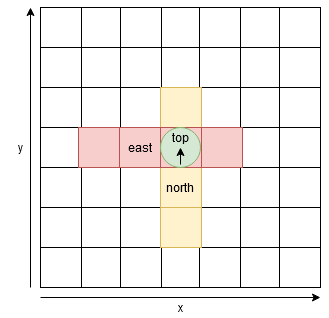
\includegraphics[width=0.5\textwidth]{stencil.png}
    \caption{2D projection of the stencil shape. The green dot symbolizes the flux in "top" direction, going along the z axis.}
    \label{fig:stencil_shape}
\end{figure}
\subsubsection{Tiled stencil computation}

\subsection{Benchmarks}
\section{Interfacing with Jax}
\label{sec:integrate}
Uses XLA
Integrating CUDA code with Cython
Needs modified compiler... blah



\bibliographystyle{alphadin}
\bibliography{main}
\end{document}
%%  ==================================================================
%%  End document
\iffalse %project description

Currently, many scientists use purely sequential software for ocean modelling, leading to long simulation times andinefficient use of modern hardware.The aim of this project is to tackle this problem by introducing highly parallel code that uses the potential of modern GPUsto accelerate the modelling process.Specifically the student will try to enhance the performance of the library Veros using massively GPUs.In this library there exist a few specific bottlenecks that significantly slow down the modelling process. For example,since the modelling process uses a grid-like structure, there is the need to quantify the effect of water turbulence thatis a lot smaller than one grid cell on the large-scale flow of the ocean.This problem and another two of the most important bottlenecks are already implemented using different performance-focused frameworks like JAX, Numba, CuPy, etc. with the aim of finding a suitably performant solution. However, thereis hope that these implementations can be improved further or that other languages like CUDA and Futhark can yieldhigher performance gains.Within the project, the student implements these bottlenecks in the GPU-accelerated languages CUDA and Futhark,aiming to achieve a solution that performs better than the existing implementations. This can potentially save a lot of timefor the scientists running the experiments and possibly also reduce the energy consumption required for the modellingprocess by using the hardware more efficiently.This involves interfacing the new implementations with the existing codebase, more specifically with the frameworkJAX, through either passing pointers to the GPU memory between the libraries or registering XLA “custom calls” withJAX. These XLA “custom calls” would allow the direct use of C++ or CUDA code (possibly generated by Futhark) withinJAX.Additionally this project requires the use of profiling tools for evaluating the performance of the implementations as wellas potentially identifying further bottlenecks in the framework.Learning Goals:• Understanding the basic structure of the ocean modelling library Veros• Efficient algorithm design in different parallel languages (CUDA/Futhark)• Identification of performance bottlenecks in parallel programs• Interfacing Futhark and CUDA implementation with existing python codebases• Using XLA custom calls to use C++/CUDA code within JAX*29/01/2021WrittenAccelerating Ocean Modelling
\fi